%
% Chapter 1
%

\chapter{INTRODUCTION}
Henri Bequerel and Marie Curie's discovery of natural, spontaneous radiation in 1896 fueled the scientific tinder that erupted into modern physics. This breakthrough in scientific impetus, coupled with the formulation of quantum mechanics and the discovery of the nucleus (the incredibly dense and miniscule core of the atom) in the early 20$^{th}$ Century, led to this brand new field of nuclear science. Initially, the nucleus was modeled as a homogenous core of positive charge, but with continued study, the nucleus was found to be comprised of discrete, $\sim$1~femtometer large (or small, depending on perspective) particles, the positively charged proton and the inert neutron, all held together with a very attractive and short-range force, the aptly named the strong interaction.

% \section{Nuclei as a Many-body Quantum System}
\label{sec:Nuclei_quantum_system}
Knowing that the atomic nucleus is comprised of protons and neutrons, we can study it as a many-body quantum system. Throughout the entirety of nuclear science's history, we have studied countless nuclear structure properties, including the nuclear (and nucleon) masses and properties of excited states in the nucleus. Several observations of phenomena like the spin and parity of the ground state of even-even nuclei being 0$^+$ led directly to the evolution of the nuclear shell model, which then drove further theories and experiments to describe the nucleus in deeper ways. The nuclear shell model saw incredible success for a great deal of nuclei, particularly at the shell closures, where the spins and parities of the second, third, and onward states agreed exceptionally well, but overall, the shell model did not see unified, complete success for all nuclei. 

% In some cases, the ratio of energies of the second and third excited states 
% The next step was to then devise a way to describe the nucleus as a liquid drop. 


By describing the nucleus as a geometric shape of a liquid drop (Equation \ref{eq:def_radius}), the nucleus can be represented as a quantum system with varying degrees of freedom about that spherical shape, by performing a multipole expansion in terms of the spherical harmonics. %manifesting as nuclear vibrations and rotations.


\begin{equation}\label{eq:def_radius}
R=R_{sp} [1+\sum_{\lambda\mu} \alpha_{\lambda\mu} Y_{\lambda\mu}(\theta,\phi)]
\end{equation}

Here, \textit{R$_{sp}$} is the average \textit{spherical} nuclear radius, often given by the well-known approximation of R$_{sp}$=R$_0$A$^{\frac{1}{3}}\approx$1.2A$^{\frac{1}{3}}$~fm. \textit{Y$_{\lambda\mu}$($\theta$,$\phi$)} represent the spherical harmonics of order $\lambda$, with corresponding expansion coefficients \textit{$\alpha_{\lambda\mu}$}. These static, permanent geometric deformations can be characterized by an expansion of their multipole order, \textit{$\lambda$}, with $\lambda$=2 being a quadrupole deformation, $\lambda$=3 as an octupole, and so on. Trivially, if $\lambda$=0, we are left with the spherical case. The lowest-order (and most common) static deformation in nuclei, the quadrupole deformation ($\lambda$=2), can be reparameterized into the Euler angles and subsequently the polar-like `Hill-Wheeler' coordinates \textit{$\beta$} and \textit{$\gamma$}, (Equations \ref{eq:Eulerangle_param1} \& \ref{eq:Eulerangle_param2}), which provides measures of the extent of quadrupole deformation and the departure from axial asymmetry, respectively. Performing this parameterization also allows us to make a convenient convention of dynamic deformation `directions' later on, as well as a categorization of the nuclear shape. So, for each axis (k=1,2,3) of our deformed solid nucleus, the deviation from spherical symmetry is given by Equation \ref{eq:Hill-Wheeler_radius}, where we also gain this categorization of the various deformed nuclear shapes based on the range of both \textit{$\beta$} and \textit{$\gamma$}. 

\begin{align}
\alpha_{2,\pm2}=\beta\sin\gamma \label{eq:Eulerangle_param1}\\
\alpha_{2,0}=\beta\cos\gamma \label{eq:Eulerangle_param2}\\
\delta R_k=\sqrt{\frac{5}{4\pi}}\beta\cos(\gamma-\frac{2\pi k}{3}) \label{eq:Hill-Wheeler_radius}
\end{align}

Figure \ref{fig:chart_nuclides} shows the Chart of Nuclides, which displays every isotope of observed nuclei with the number of protons (Z) on the y-axis and the number of neutrons (N) on the x-axis. In this plot, the R$_{\frac{4}{2}}$ values (the ratio of the energies of the first 4$^+$ state to the 2$^+$ state) for even-Z/even-N nuclei are shown as a color gradient; this R$_{\frac{4}{2}}$ ratio is a practical measure of static deformation in the nucleus, with shades of orange ($>$3) representing well-deformed nuclei and shades of green ($<$2) representing spherical or near-spherical shape. Throughout the region of deformation (and the entire Nuclear Chart), experimental physicists have observed the various emergent nuclear phenomena of vibrations and rotations to drive experiments and theories further.

\begin{figure}[h!] 
\begin{center}
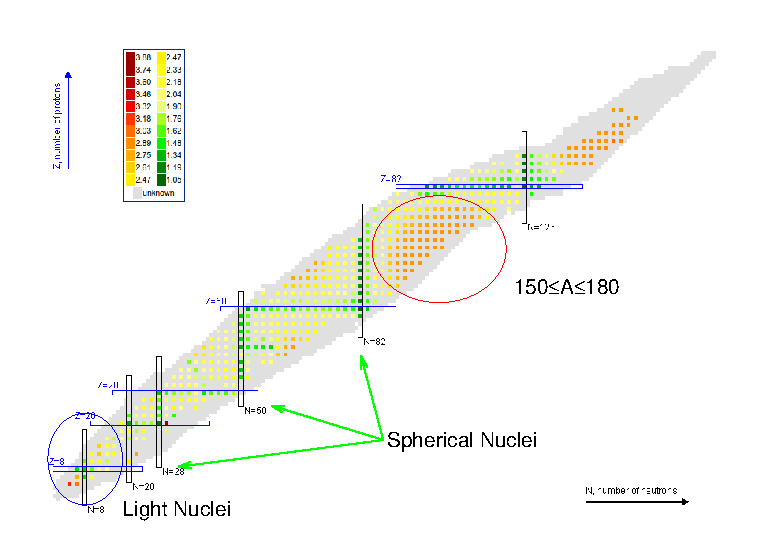
\includegraphics[width=\textwidth]{figures/Chart_of_Nuclides_def.eps}
\caption{Chart of nuclides showing the varying degrees of deformation (R$_\frac{4}{2}$ values for even-even nuclei). Orange colored squares mark a well-deformed ground state, with green representing spherical nuclei.}
\label{fig:chart_nuclides}
\end{center}
\end{figure}
% \newpage

The first such phenomenon is the existence of small surface oscillations of spherical nuclei, in which the nucleus can exhibit a macroscopic, collective motion of nucleons about the spherical equilibrium shape. These vibrations about the spherical shape are well-documented and studied throughout the spherical mass ranges of the Chart of Nuclides as an excellent example of collective degrees of freedom in the nucleus \cite{Casten_text,Aprahamian_118Cd}. These vibrational quanta, or phonons, also manifest in higher-order excitations (a two-phonon vibration, a three-phonon vibration, etc) as superimposed vibrations built on top of other vibrations.

Vibrations, however, are not the only collective degree of freedom afforded to the nucleons in the nucleus; collective rotations of nucleons about an axis are abundant in nuclei \cite{Casten_text,Wong_text}. For spherical nuclei, a nuclear rotation is energy degenerate, as there is no change in the fundamental frequency of oscillation, but in deformed nuclei, we find strong experimental evidence of collective rotations about the different axes. Whenever a quadrupole deformed nucleus rotates about an axis, it will emit electric quadrupole radiation (E2 type radiation) \cite{Rowe_Wood_text}. We subsequently observe this strong rotational motion in the transition probabilities between nuclear states (B(E2) measurements expressed in terms of a single-particle estimate) in Figure \ref{fig:nucl_rotation}, where the entire region of deformation exhibits strong ($>$50~Weisskopf unit strength) transitions, a very strong indication of collective motion.

An open question then arises: are there superimposed vibrations on top of a deformed ground state, much like the vibrations about a spherical shape?

\begin{figure}[h!]
\centering
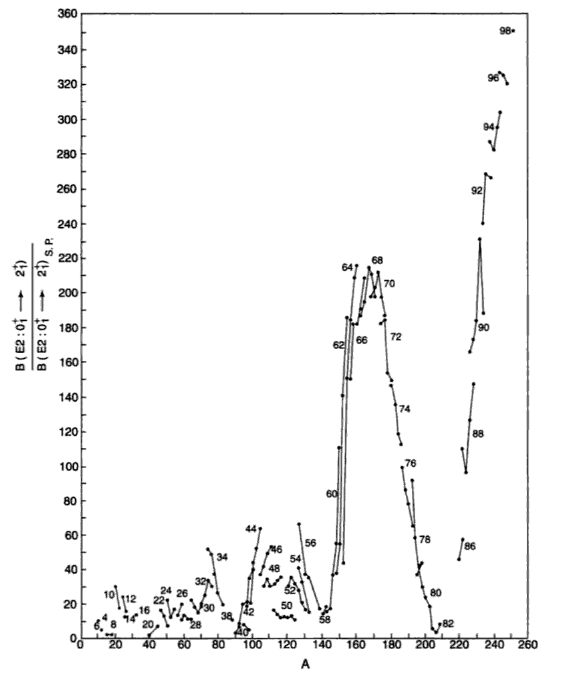
\includegraphics[width=0.95\textwidth]{figures/B(E2)_rotations_Casten.png}
\caption{Measured B(E2) transition probabilities in single-particle units as a function of A, highlighting the region of deformation (as well as heavier actinide region) where strong nuclear rotations exist \cite{Casten_text}. \label{fig:nucl_rotation}}
\end{figure}
\newpage



% From this qualitative picture, we can observe several nuclear structure phenomena at a glance. Immediately, we see the \textit{magic} nuclei, incredibly well-bound and stable nuclei where Z or N are equal to 2, 8, 20, 28, 50, 82, or 126. This is an effect of the nuclear shell model (an analogue to the atomic electron shell model), where nuclei will fill sequential, discrete shells with nucleons, which can be used to determine properties of the nucleus by examining which shells are filled (or unfilled) with either protons or neutrons. We can represent the structure of the very light nuclei (fewer than $\sim$20 nucleons), as well as the nuclei near shell closures, with models like the nuclear shell model. However, the shell model begins to lose its applicability and interpretability as we add larger numbers of nucleons to the system, and as the nuclear ground state becomes less spherical.

\section{Deformation in Nuclei}\label{sec:nuclear_deformation}
% Spherical nuclei behave quite predictably under the shell model, yet as we stray farther away from the closed shells at the magic numbers and into the realm of deformed nuclei, this model begins to break down and becomes extremely (if not impossibly) complicated and computationally intensive. For perspective, ``To quote the famous example of Talmi, in $^{154}_{62}$Sm$_{92}$, approximately 3$\times$10$^{14}$ [J$^\pi$=]2$^+$ states can be constructed with" its combination of protons and neutrons via shell model considerations \cite{Casten_text}. The gravity behind this statement should not be understated, as the Samarium-154 nucleus contains a \textit{modest} number of nucleons, even in comparison to the similarly deformed nucleus, yet significantly more massive, $^{184}_{74}$W$_{110}$. If we are to realistically model the structure of nuclei (most of which are \textit{not} spherical, especially above A$\approx$20), more exotic methods must be implemented by expanding the microscopic nature of particle-hole excitations in the nucleus. This is done by introducing pairing correlations into the nuclear wavefunctions, in a departure from the single-particle nature of the shell model. 

%rotational nuclei, deformed ground state

Description of collective motion for a deformed nucleus begins by treating the nuclear radius as a liquid drop with the statically deformed shape shown in Equation \ref{eq:def_radius}, and then allowing the deformation parameters to deviate in small amplitudes. The work contained in this dissertation is strictly concerned with static, prolately deformed nuclei, or where $\gamma$=0 and $\beta>$0, although other nuclear shapes exist for negative values of $\beta$ (oblate, axially asymmetric, etc). This deformed nuclear shape is equivalent to a permanent quadrupole deformation in the ground state, or where $\lambda$=2 from Equation \ref{eq:def_radius}. It is also convenient and prudent to recast the angular momentum of states in the deformed nucleus as a projection of the total angular momentum along the axis of symmetry (K$^\pi$); this is beneficial, as it helps us easily identify and distinguish the different types of collective motion in deformed nuclei. K$^\pi$ can further be distinguished by the parity of states, as is typical by a $\pi$=(-1)$^\lambda$ rule, where this is also a clue to the asymmetry of nuclear wave functions.


Effects due to the pairing of nucleons in discrete shells and subshells in the nucleus have a profound effect on the structure of states in the deformed nucleus. In one of the most important pairing effects, the pairing of fermions in discrete shells forbids particles from occupying the same space, so when two protons or neutrons pair together to create an excitation (or as the even-even nucleus resides in the ground state). However, there is an energy intrinsic to the nucleus at which two nucleons will break their tendency to couple together as pairs; this pairing gap for protons and neutrons (2$\Delta_{\pi}$ \& 2$\Delta_{\nu}$ respectively) is taken from \cite{MANG_pairing1965353}, and is a measure of the odd-even staggering of energies caused by the pairing interaction in the nuclear binding energy. In the rare-earth region of nuclei, this pairing gap is experimentally observed near $\sim$1.5-2.0~MeV, where the states below this energy are the signatures of macroscopic collective motion of nucleons (or in terms of pairing, multiple quasiparticle pairs acting in the form of vibrational phonons) as a whole, in a dramatic shift away from independent/single particle excitations \cite{Bohr_pairing1958}. These pairing effects then bring rise to the idea of nuclear excitations being created via quasiparticle pairs; this is stated in stark contrast to the rigid rules of the shell model where fermions (in the case of particle-hole states) will have defined occupancy of shells, and instead can exhibit partial occupancies. Above the pairing gap, we notice a sharp increase in level density, where we have state-mixing occurring between the particle, quasiparticle pair, and collective configurations, and as such, finding a `pure' collective vibration becomes increasingly difficult \cite{Casten_text,Heyde_text}.


% The energies of quasiparticle excitations simplifies the picture of the shell model immensely, in that these energies are expressed relative to the absolute Fermi energy, which condenses the entire occupancy of the shell model down to a few excitations relative to this Fermi surface \cite{Casten_text}. 
% Since the quasiparticle energies are constructed with respect to the pairing gap 2$\Delta$, we can see experimental evidence of this pairing gap, which affects the level density, the sphericity of surface shape, and the microscopic character of states \cite{Casten_text}. With this key dinstinction between collective and single particle interactions in mind, the collectivity of states, not only below the pairing gap, but across the entire continuum of nuclear states is of paramount importance.  %The role pairing has on the nuclear excitation is that coherent pairs of nucleons cannot be formed above this gap, meaning the states above the gap \textit{cannot} be attributed to pair correlations. Any states below the pairing gap are surmised to be macroscopic collective vibrations. Data in the literature points to very few two-particle excitations below the pairing gap of any particular nucleus. 

The pairing gap for a particular nucleus $^A_Z$X$_N$ can be calculated with Equations \ref{eq:pairing_gapP} and \ref{eq:pairing_gapN} (\cite{MANG_pairing1965353}), where E(N,Z) is the binding energy of the nucleus X for the particular neutron number N and proton number Z combination, and E(N,Z+1) is the binding energy of a nucleus that has an added proton, E(N,Z+3) is the nuclear binding energy of the nucleus with three added protons, and so on. For example, the proton pairing gap for $^{162}$Dy would involve the binding energies of $^{162}$Dy, $^{163}$Ho, $^{165}$Tm, $^{161}$Tb, and $^{159}$Eu, for the respective entries in Equation \ref{eq:pairing_gapP}.

\begin{align}
2\Delta_{\pi}=\frac{1}{8}[16E(N,Z)+9E(N,Z+1)+E(N,Z+3)+9E(N,Z-1)+E(N,Z-3)] \label{eq:pairing_gapP}\\
2\Delta_{\nu}=\frac{1}{8}[16E(N,Z)+9E(N+1,Z)+E(N+3,Z)+9E(N-1,Z)+E(N-3,Z)] \label{eq:pairing_gapN}
\end{align}

\subsection{Vibrations in Deformed Nuclei}
Given some excitation energy, the deformed nucleus' excitations are not necessarily treated as single particle excitations, but instead as a movement of multiple nucleons \textit{collectively} (as a whole) throughout the nuclear shape as it rotates. In the mid-20$^{th}$ Century, theoretical treatments to describe a deformed nucleus emerged as the geometric collective model of Bohr and Mottelson \cite{BohrMott_text}, and one of the beauties of of this descriptive model was the near-immediate appearance of low-lying surface oscillations (in this case, nuclear vibrations) about the deformed ground shape \cite{BohrMott_text}, as well as the prevalence of fundamental nuclear rotations. These two modes of collective motion, vibration and rotation, make up the basic degrees of freedom available to a deformed nucleus, where, in stark contrast to the degenerate vibrations of a spherical nucleus, a vibration in a deformed nucleus can be along any of the axes of symmetry according to a time-dependent multipole expansion of the deformed shape. In its lowest order ($\lambda$=2 expansion of Equation \ref{eq:def_radius}), the nucleus \textit{can} exhibit quadrupole oscillations around its equilibrium shape in one of two possible types, a $\gamma$-vibration or a $\beta$-vibration. The notation and phenomenology behind these modes of vibrations alludes to the `direction' of oscillation with respect to the Hill-Wheeler coordinate parameterization mentioned earlier in \S\ref{sec:Nuclei_quantum_system}. For example, the $\gamma$-vibration is a dynamic oscillation that breaks axial symmetry (the parameter $\gamma$) to maintain a K$^\pi$=2$^+$ projection of angular momentum, while the $\beta$-vibration (an oscillation of quadrupole deformation $\beta$) maintains both axial symmetry, as well as a K$^\pi$=0$^+$ projection of angular momentum. Note the positive parity, which indicates a reflection symmetry for the nuclear shape and corresponding wave functions. Crude cartoon visualizations of these quadrupole vibrations can be seen in Figures \ref{fig:beta_vibration} and \ref{fig:gamma_vibration}. In these pictures, the schematic on the left looks down the axis of symmetry (represented by bold, black lines), with the side view on the right. Thin black lines outline the deformed equilibrium shape, with dashed red lines showing the extent of the dynamic, quadrupole oscillations; blue arrows are meant to guide the eye as to how the nucleus changes shape. 

\begin{figure}[h!] 
\begin{center}
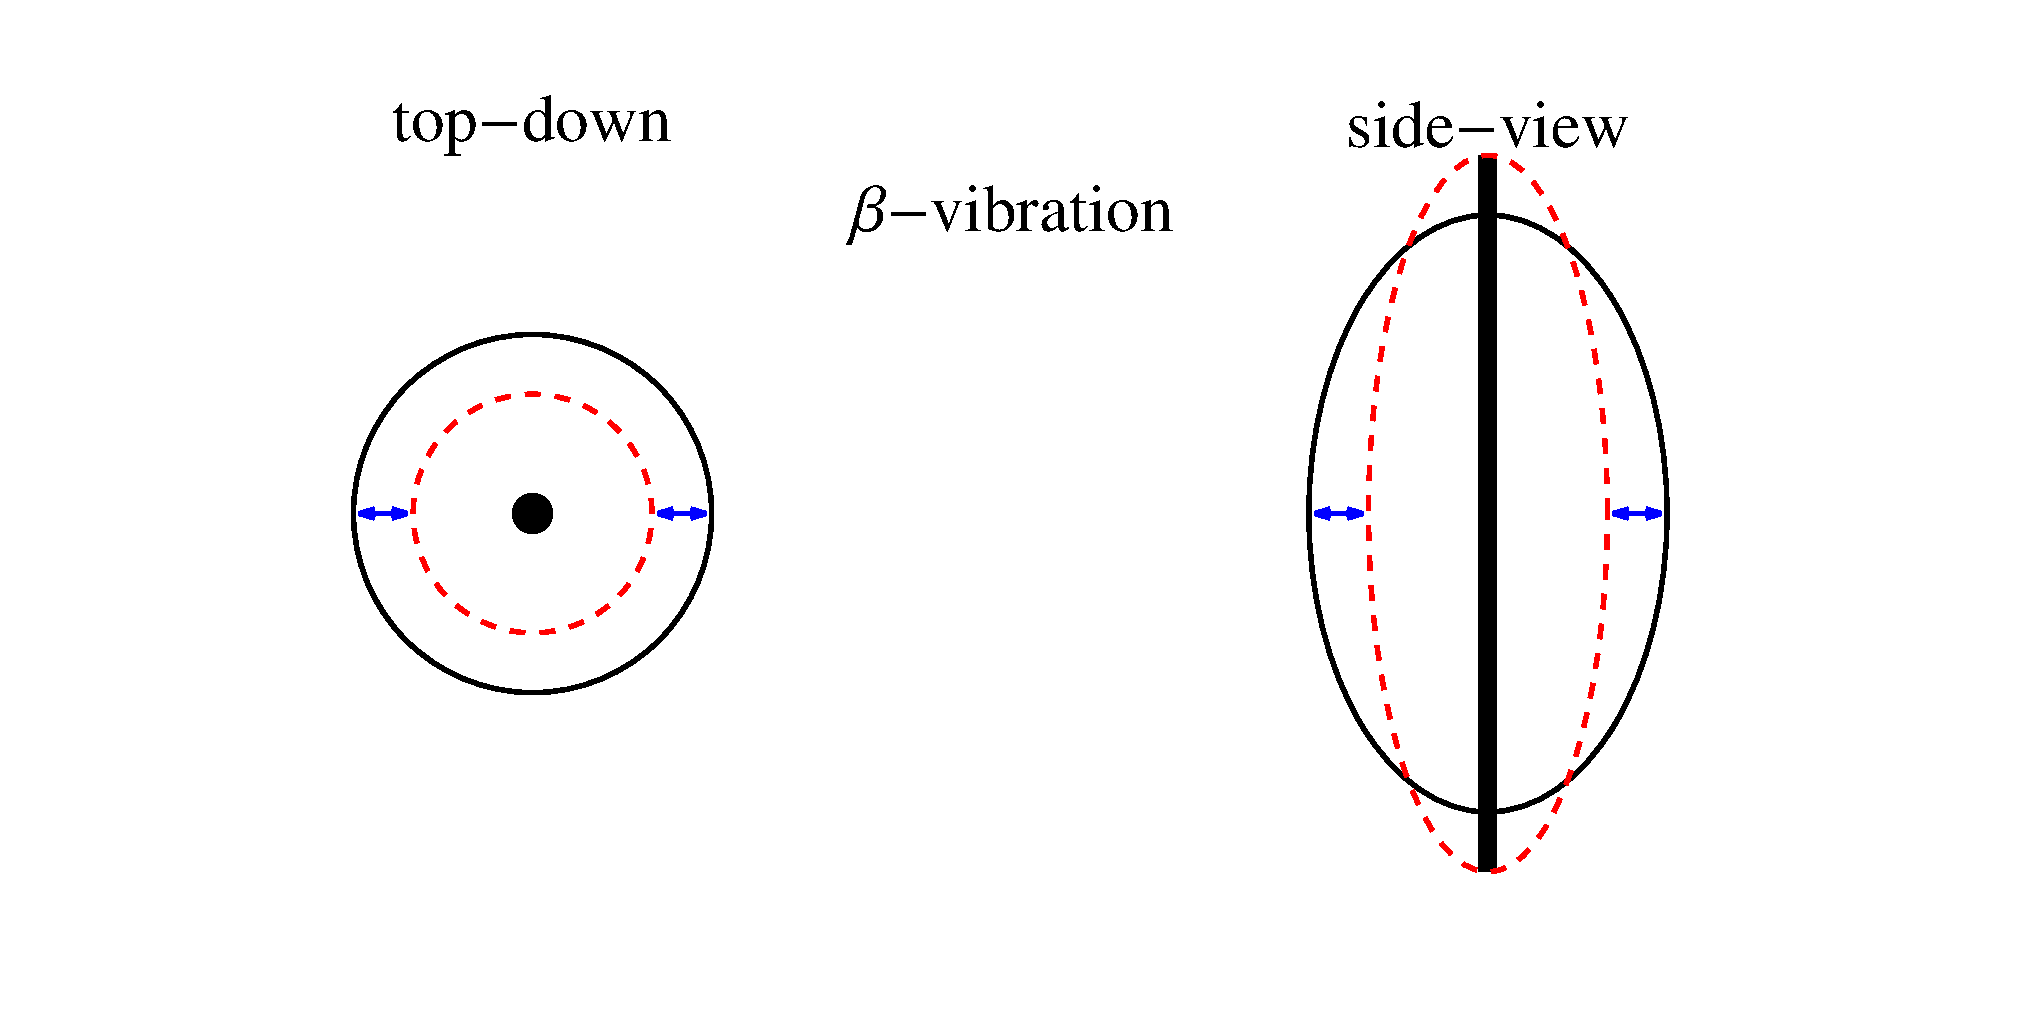
\includegraphics[width=\textwidth]{figures/SciDraw_beta_vibration.eps}
\caption{Schematic of the $\beta$ quadrupole vibration about a deformed equilibrium shape.}
\label{fig:beta_vibration}
\end{center}
\end{figure}

\begin{figure}[h!] 
\begin{center}
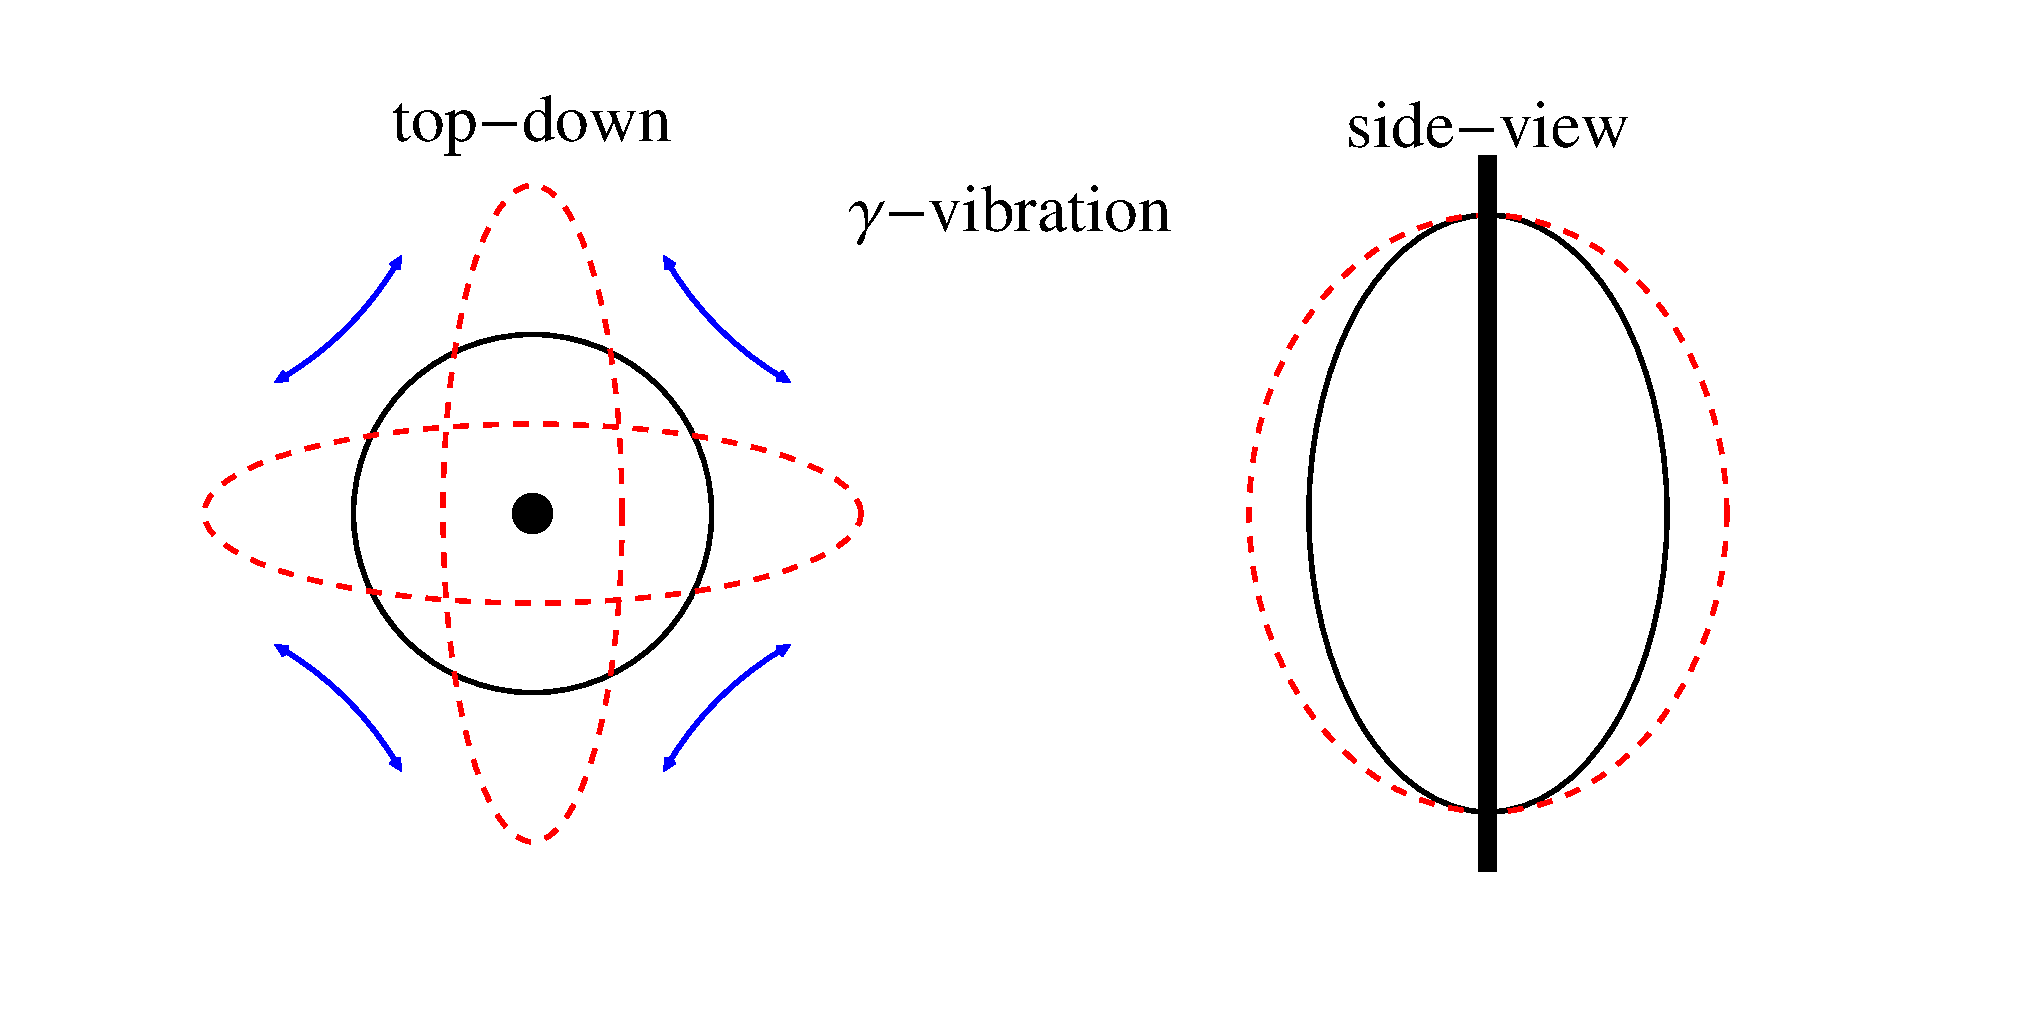
\includegraphics[width=\textwidth]{figures/SciDraw_gamma_vibration.eps}
\caption{Schematic of the $\gamma$ quadrupole vibration about a deformed equilibrium shape.}
\label{fig:gamma_vibration}
\end{center}
\end{figure}

If a single vibrational phonon can be superimposed on the collective rotational ground state, how feasable is the two-phonon case for deformed nuclei? Linear combinations of the quadrupole phonon structure would involve the $\gamma\gamma$ (with either a 0$^+$ or 4$^+$ K$^\pi$ projection), $\beta\gamma$ (K$^\pi$=2$^+$), \& $\beta\beta$ vibrations (again, K$^\pi$=0$^+$). As an analogue to the classical harmonic oscillator problem, the addition of multiple phonon quanta will increase the energy of the system by some proportional amount, so we would expect a 2 phonon vibration to be double the energy of the 1 phonon vibration, or that E$_{phonon}\propto$N$_{phonon}$. \textit{In theory}, all modes of vibration should be obvious and abundant, but we will see that this is not immediately the case for deformed rare-earth nuclei given the current state of experimental data, especially with varying degrees of anharmonicity at play.

A further study in deformed nuclei is on the higher order octupole ($\lambda$=3 expansions of Equation \ref{eq:def_radius}) vibrations and if they can also exist, but the motions of the nuclear surface are significantly more difficult to envision as a drawing, especially on a 2-dimensional piece of paper. However, qualitatively, the octupole vibration is an asymmetric vibration about the quadrupole deformed nucleus in a `pear'-like oscillation. The octupole vibration (in deformed nuclei) manifests as a K$^\pi$=3$^-$ projection on the axis of symmetry, with asymmetric wave functions (and shape) due to the negative parity. However, in contrast to the degenerate quadrupole modes of K=0,2 in deformed nuclei, we expect a split-degeneracy of this K$^\pi$=3$^-$ projection into a quartet of possible projections, K$^\pi$=0$^-$, 1$^-$, 2$^-$, and 3$^-$ \cite{BohrMott_text} in the deformed nucleus.

%[PHONON EXPLANATION SOMEWHERE!!!!]
%really need to lay out some base for the phonon structure, energetics, etc
% The collective model is a purely geometric model of the behavior of nuclei, but is only broadly applicable in a moderate range of deformed nuclei. Alternative theories exist in an attempt to formulate a unified theory of structure that spans the bulk of the Chart of Nuclides, even in contrast to the somewhat limited scope of the shell model and geometric collective model. Beyond this traditional Bohr and Mottelson formalism, evolution of nuclear structure studies erupted in the early 1970s with Lie Algebraical based formulations.
%, even in contrast to the shell-model and geometric collective model.

% Iachello and Arima devised the Interacting Boson Approximation (IBA) to exploit the power of algebraic groups to model quantum systems, like the atomic nucleus. Exact symmetries from the set of algebraic groups can describe nuclear structure phenomena such as excitation energies, reduced transition probabilities, and branching ratios, very quickly and and with widespread success. An elegant treatment, the IBA models the nucleus' valence nucleons as aggregate pairs of \textit{s} and \textit{d} bosons, with L=0 and L=2, respectively; the set of all substates of boson, the single monopole and five non-degenerate quadrupole bosons (\textit{s}, \textit{d$_{-2}$}, \textit{d$_{-1}$}, \textit{d$_{0}$}, \textit{d$_{1}$}, and \textit{d$_{2}$}) span a 6-dimensional space, represented by the unitary Lie Algebra group U(6). The decomposition of the U(6) group into the triplet subgroups of U(5), SU(3), \& O(6) lays down the framework to describe fundamental properties of nuclei. Each subgroup describes a separate `category' of nuclei, with textbook examples of nuclei that exhibit analogues to the expected geometrical behavior, with U(5) representing a purely harmonic vibrator, O(6) providing symmetries to describe an axially asymmetric `$\gamma$-soft' nucleus, and SU(3) gives rise to the deformed rotor. Each of these symmetries gives rise to irreduceable representations within the IBA, from which, we can make statements about the structure of states in the nucleus.
%Each subgroup contains distinct properties about the nucleus, including expected energies of excited states, transition probabilities between states, as well as selection rules for decays 
% The IBA is not without its limitations, the basis states set up by each subgroup cannot perfectly reproduce the specific nuclear structure of most nuclei, but at the very least, it provides a baseline understanding of structure.

% By forming the nuclear Hamiltonian ($\mathcal{H}\Psi=E\Psi$) in terms of the s or d boson creation and annihilation operators ($s^\dagger$, $\tilde{s}$, $d^\dagger$, $\tilde{d}$), we can write the standard IBA Hamiltonian as Equations \ref{eq:IBA_H} and \ref{eq:IBA_Q}. The structure that arises from one of the three subgroups is referred to as a \textit{dynamical symmetry} \cite{Casten_text}, where each symmetry contains distinct properties about the nucleus, including expected energies of excited states, transition probabilities between states, as well as selection rules for decays. For example, the extreme limiting case of the SU(3) symmetry states that the lowest K=0,2 bands stem from the same irreduceable representation, and as such, strong transitions from these states cannot be connected to the ground state band \cite{Casten_text}. We will find that in many cases, using the strict limits of each symmetry offers very little room for flexibility in a realistic, nuclear system. So from here, we can easily represent nuclei belonging to the three dynamical symmetries by this three parameter space, $\varepsilon$, $\kappa$, and $\chi$. Calculations for any nucleus can now be done by varying one or more of these parameters, with extreme ease, and without adding needless complexity to the system.
% \begin{align}
% \mathcal{H}(\varepsilon,\chi,\kappa)=\varepsilon n_d+\kappa\mathcal{Q}\cdot\mathcal{Q}\label{eq:IBA_H}\\
% \mathcal{Q}=s^\dagger\tilde{d}+d^\dagger\tilde{s}+\chi[d^\dagger\tilde{d}]^2\label{eq:IBA_Q}
% %\frac{\varepsilon}{\kappa}=4N\frac{1-\zeta}{\zeta}\label{eq:IBA_param}
% \end{align}

% A useful way to visualize the parameter space that describes U(5), SU(3), and O(6) nuclei is best seen in the IBA Symmetry Triangle, seen in Figure \ref{fig:Casten_Triangle}. This Symmetry Triangle maps out the parameter space of $\varepsilon$, $\kappa$, and $\chi$ that correspond to the limits of the different U(6) symmetries. However, this implies that nuclei do not have to ascribe to the very rigid limits of any particular symmetry (this is generally the case for most nuclei); `transitional' approaches must be made, where the open parameters for each symmetry become intermediate values along the `legs' or `arcs' in the IBA symmetry triangle (Figure \ref{fig:Casten_Triangle}). 
% 
% Physical phenomena are kept close at hand with the IBA with this low-parameter model; on a general scale with the IBA Hamiltonian (Equation \ref{eq:IBA_H}), we can attribute the first term, $\varepsilon n_d$, to the a spherical shape and structure, with any physics that determines deformation governed by the $\kappa\mathcal{Q}\cdot\mathcal{Q}$ term. One of the fundamental aspects of nuclear structure inside the IBA Hamiltonian (and throughout most models) is the importance of E2 transitions, in this case, simply related to $\mathcal{Q}$ by Equation \ref{eq:IBA_E2}, where e$_B$ is an effective boson charge \cite{Casten_text}.
% \begin{equation}\label{eq:IBA_E2}
% \mathcal{T}(E2)=e_B\mathcal{Q}
% \end{equation}

% These simplistic approaches to describing nuclear structure phenomena are a common theme with the IBA, by keeping the physics represented by the algebraic symmetries very accessible, while also providing limiting cases of `ideal' behavior from any of the pure dynamical symmetries.
%cite a bunch of IBA papers in the field here

%SU(3) is too strict (Casten 278)
%[IBA 1969-1975]
%PUBLISHED IN 87

%SHOULD ONLY HAVE TO GO INTO DETAIL ABOUT SU(3)
% \begin{figure}[h!] 
% \begin{center}
% 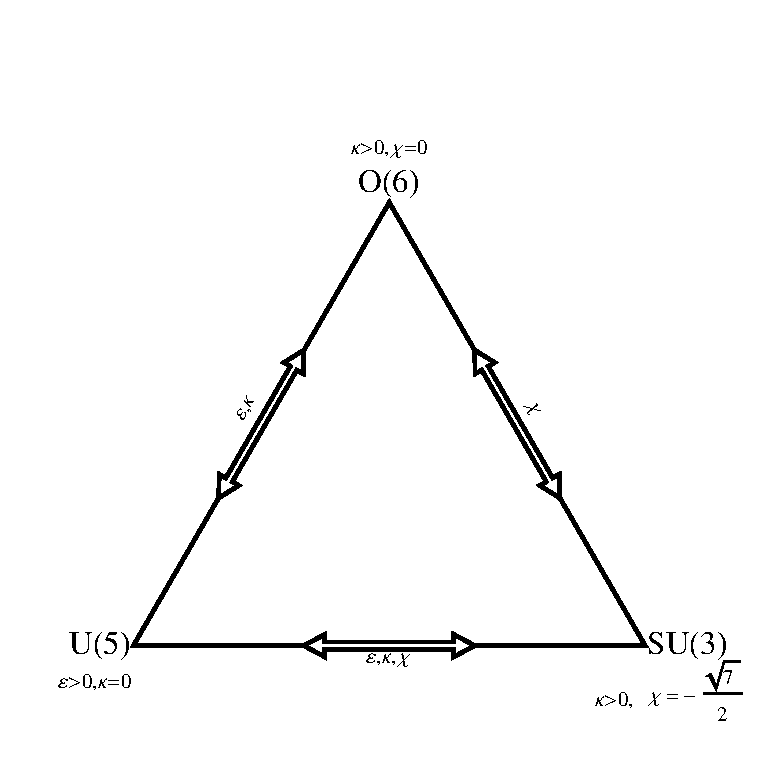
\includegraphics[width=\textwidth]{Casten_Triangle.eps}
% \caption{IBA triangle containing SU(3), U(5), \& O(6) symmetry limits with corresponding $\varepsilon$, $\kappa$, and $\chi$ parameters. Arrows on the `legs' of the triangle indicate which parameters are varied to perform a transitional nucleus' calculation.}
% \label{fig:Casten_Triangle}
% \end{center}
% \end{figure}

%IBA+F boson to take care of negative parity states (Barfield ref)
\section{Excited States in Deformed Nuclei}\label{sec:excitedstates}
The question then arises: what would these quadrupole and octupole vibrations look like represented as low-lying excited states in the level scheme of a well-deformed rotational nucleus? A cartoon level scheme representing the lowest lying quadrupole and octupole vibrations is given in Figure \ref{fig:phonon_def}, where we can immediately see the ensemble of states corresponding to each vibration, and each vertical `band' lines up with rotational members a particular vibrational state. Starting in the bottom left, we see the low-lying K$^\pi$=2$^+$ and 0$^+$ bands as the $\gamma$ and $\beta$-vibration (where one would expect near $\sim$1~MeV excitation energy). Then, continuing upward, the single-phonon vibrations of $\gamma$ and $\beta$ type have their corresponding two-phonon counterparts and combinations ($\beta\beta$, $\beta\gamma$, and $\gamma\gamma$) drawn at twice the excitation energy that assumes a completely harmonic vibration.

\begin{figure}[h!] 
\begin{center}
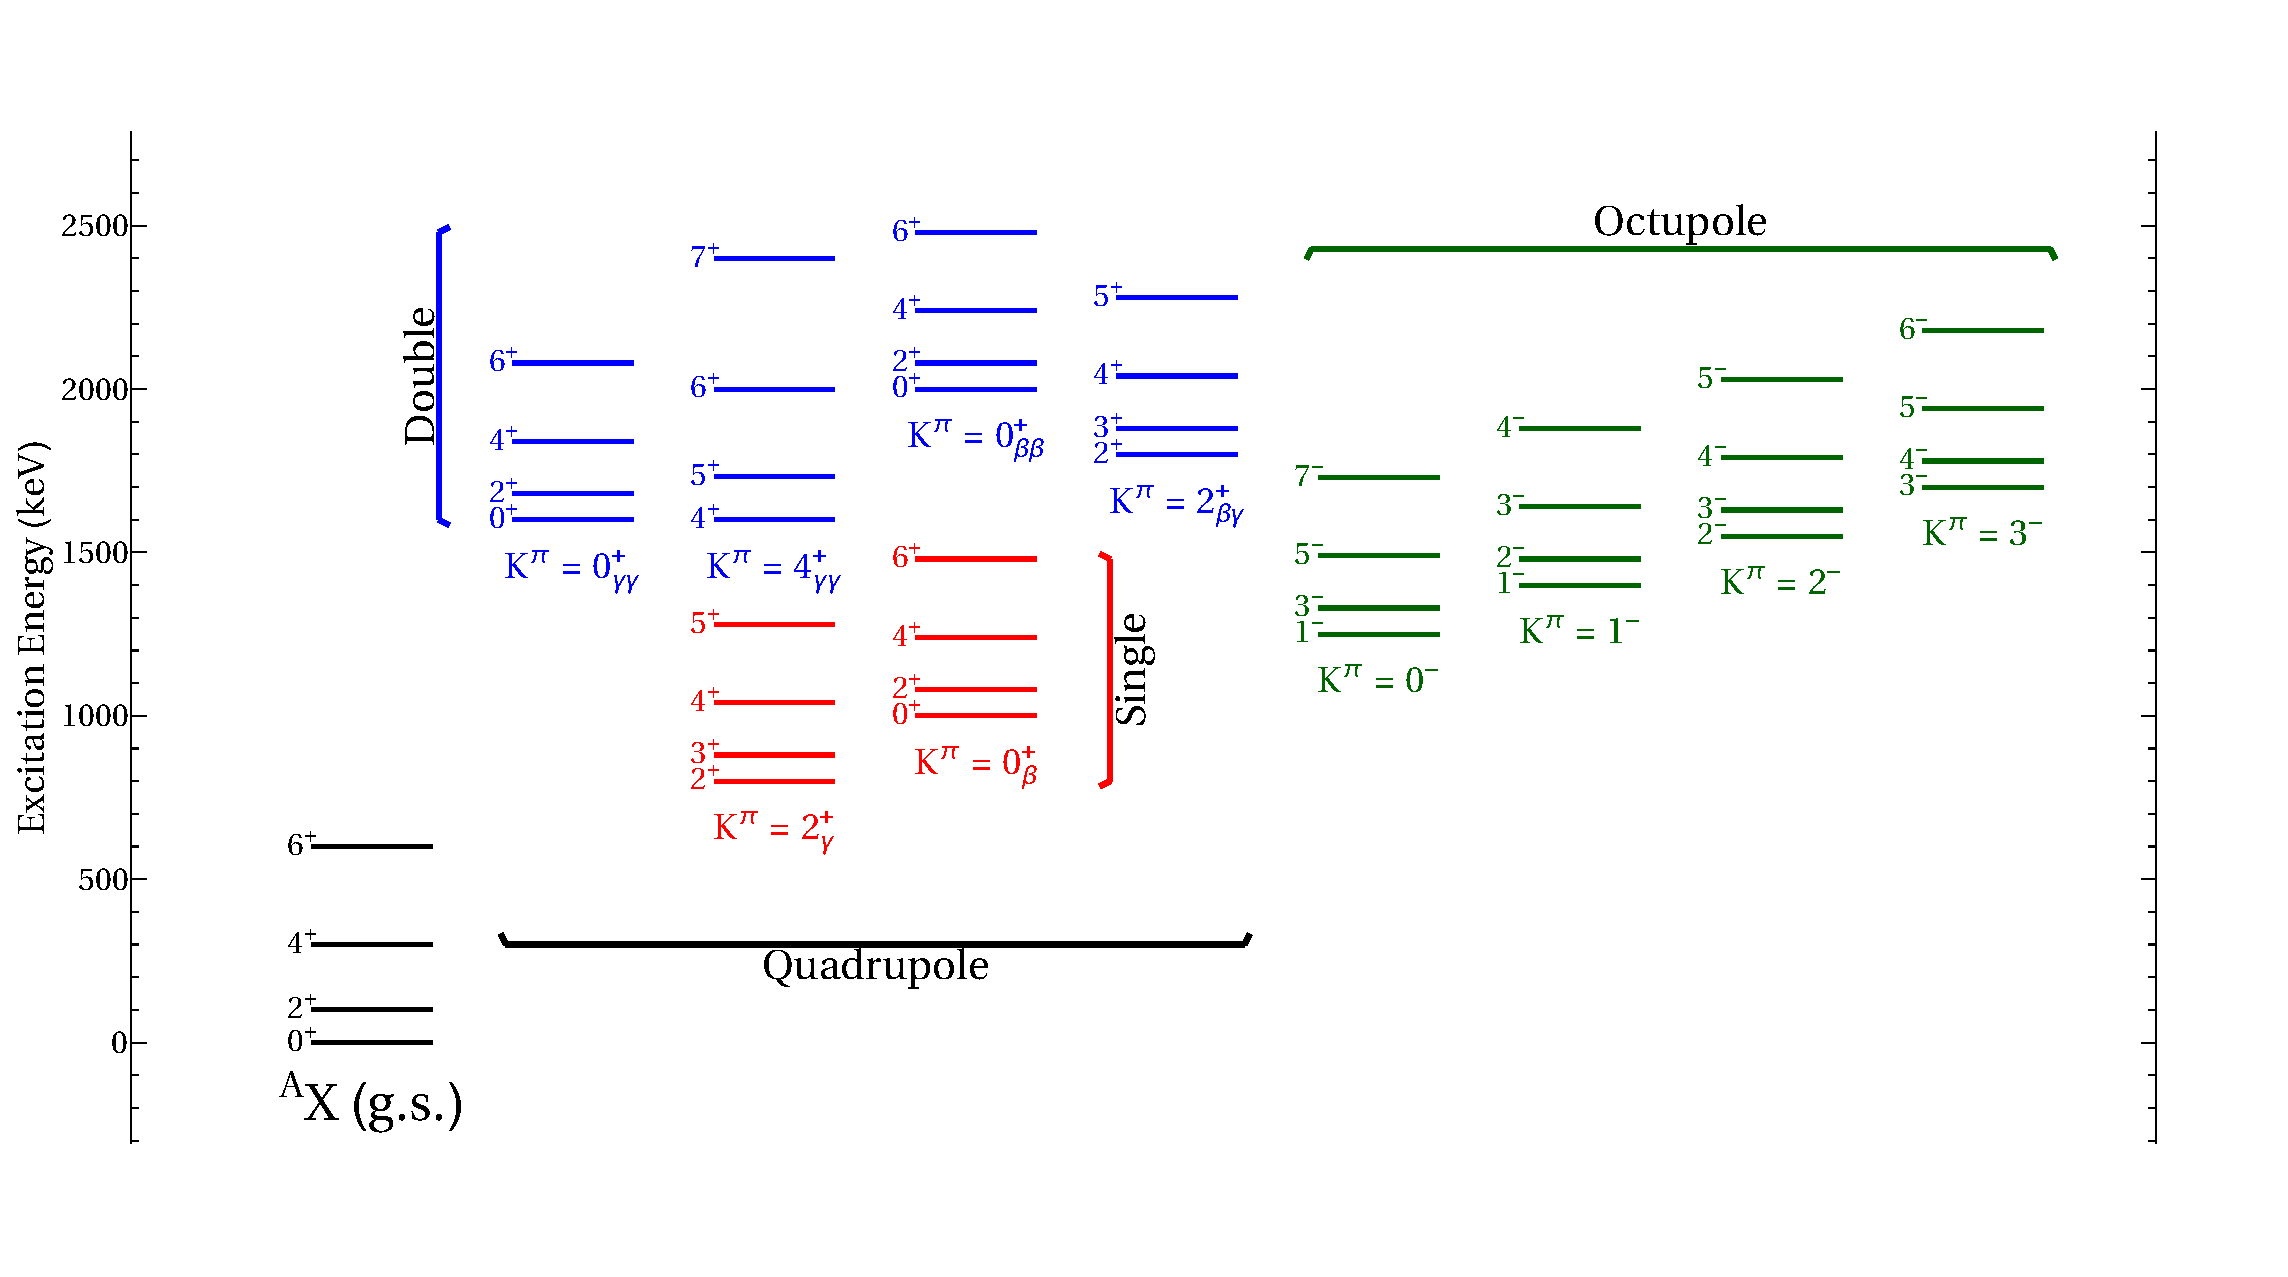
\includegraphics[width=\textwidth]{figures/phonon_deformed.pdf}
\caption{Schematic level scheme of the single- and double-phonon vibrational (quadrupole and octupole) bands expected in deformed nuclei (color online).}
\label{fig:phonon_def}
\end{center}
\end{figure}

Nuclear rotations are superimposed on the base vibration expected for each type of phonon as band excitations, (single quadrupole/octupole and double quadrupole) according to the J(J+1) rule set out in Equation \ref{eq:rotation} for low values of K, of which would include the single- and double-phonon vibrational states (K=0,2,4). These additions of rotational energy directly correlate to higher-lying members of a band, with $\mathcal{I}$ being the moment of inertia for the nucleus. The rotational excitations in a band carry a set of spins related to the band's value of K; for K$\neq$0, J progresses through K,K+1,K+2... where only even (or odd for a negative parity K=0 band) spins occur in a K=0 band \cite{Greiner_Maruhn_text}.

\begin{equation}\label{eq:rotation}
E_{rot}=\frac{\hbar}{2\mathcal{I}}[J(J+1)] % for low values of K, at least
\end{equation}

% The lowest lying state of a particular band will (with the exception of a K$^\pi$=0$^-$ band) always have J$^\pi$=K$^\pi$ (\textit{e.g.} the bandhead of the K$^\pi$=0$^+$ band will be a J$^\pi$=0$^+$ excitation), where the spins and parities of other members (the superimposed rotations) of the band are selected by the selection rules outlined in Table \ref{tab:JK_selection}. In short, K$^\pi$=0$^\pm$ will contain \textit{every other} spin-parity, while any other projection of K simply counts up J$^\pi$ from the bandhead value. For example, a K$^\pi$=0$^+$ band will have J$^\pi$=0$^+$, 2$^+$, 4$^+$ (and so on) members, a K$^\pi$=0$^-$ band will contain similarly structured 1$^-$, 3$^-$, 5$^-$ (\textit{ad infinitum}) members, where a K$^\pi$=7$^+$ band has 7$^+$, 8$^+$, and so on.
% 
% \begin{table}[h!]
% \centering
% \begin{tabular}{r|c|c|c}
% & K$^\pi$=0$^+$ & K$^\pi$=0$^-$ & K$^\pi\neq$0$^\pm$ \\
% \hline
% \hline
% J$^\pi_0$= & K$^+$ & (K+1)$^-$ & K$^\pm$  \\ 
% \hline
% J$^\pi_1$= & (K+2)$^+$ & (K+3)$^-$ & (K+1)$^\pm$  \\ 
% \hline
% J$^\pi_2$= & (K+4)$^+$ & (K+5)$^-$ & (K+2)$^\pm$  \\ 
% \hline
% $\vdots$ & $\vdots$ & $\vdots$ & $\vdots$  \\ 
% \end{tabular}
% \caption{Selection rules used to determine J$^\pi$ values of rotational members of a specific K$^\pi$ band. \label{tab:JK_selection}} %    
% \end{table}

In Figure \ref{fig:phonon_def}, we immediately see a key (and long-lived) question in nuclear structure physics: What are the nature of 0$^+$ excitations? From this ideal, toy picture, we already see three possible ways to make a K$^\pi$=0$^+$ excitation. Understanding the nature of these common, low-lying excitations in nuclei has been a cornerstone of nuclear structure in the rare-earth region for decades. Experimentally, the searches for the nature of 0$^+$ have been cloudy from the evidence of double-phonon states across the entire rare-earth region such as the $\gamma\gamma$-type vibration in several nuclei (\cite{Garrett_twogammaEr_1997}, \cite{Lehmann_doublegamma168Er_1998}, \cite{Aprahamian2002}) that exhibit strongly collective, anti-aligned combinations of the $\gamma$-vibrational phonon.

%%%%%%%%%%
Experimentally, many deformed rare-earth nuclei exhibit a low-lying excited K$^\pi$=0$^+$ and K$^\pi$=2$^+$ band, and were assumed to be the $\beta$ and $\gamma$ vibration, respectively. In practice, however, this assumption of vibrational character has come under fire in recent years and tends to fall apart due to several factors. First, we do not have a complete, unambiguous characterization of each 0$^+$ state in the rare-earth region as a collective $\beta$-vibration; this stems from a lack of lifetime information (and thus transition probability information) of the K$^\pi$=0$^+$ bands in rare-earth nuclei.

\begin{figure}[h!]
\begin{center}
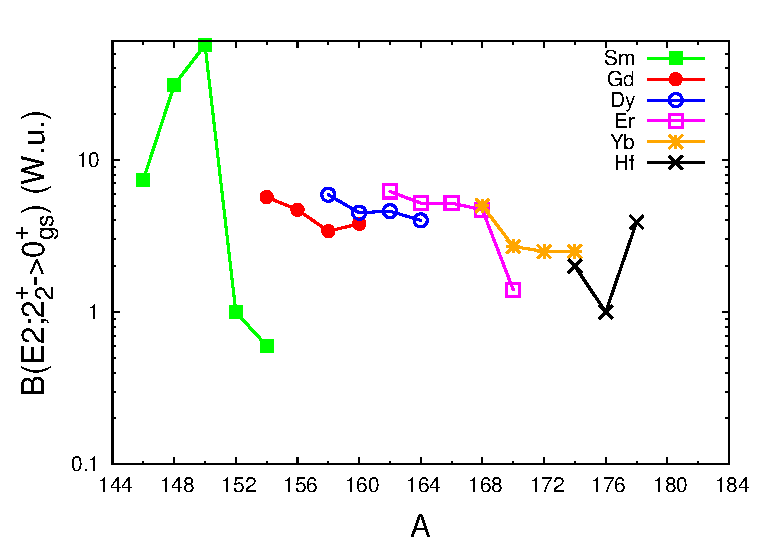
\includegraphics[width=0.88\textwidth]{figures/Rare_Earth_2g_BE2.eps}\\
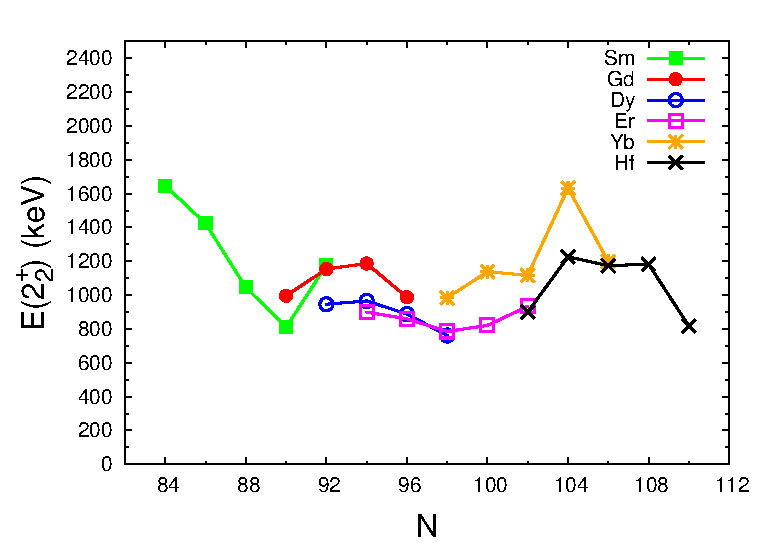
\includegraphics[width=0.88\textwidth]{figures/Rare_Earth_2g_N.eps}
\end{center}
\caption{Absolute B(E2;2$^+_\gamma\rightarrow$0$^+_{gs}$) (in Weisskopf units) measurements for rare-earth nuclei, showing the uniformity of the $\gamma$-vibration in a deformed nucleus. The bottom plot shows the energy of the 2$^+$ bandheads as a function of N, highlighting the smoothly varying energies. \label{fig:Rare_Earth_2g_BE2}}
\end{figure}

Second, examination of the B(E2) transition probabilities and energies of the lowest-lying 0$^+$ and 2$^+$ bands yields a contrasted picture for each (assumed to be) vibrational type, shown in Figures \ref{fig:Rare_Earth_2g_BE2} and \ref{fig:Rare_Earth_02_BE2}. In the case of $\gamma$-vibrational characteristics, we observe a smoothly varying energies across the entire region, with the same behavior for the overall collectivity of these states (falling around 5~Weisskopf unit strength). However, the $\beta$-vibrational systematics become quickly obscured, with both obvious gaps in the lifetime information, an order of magnitude variance of the transition probabilties, and a less than smooth variance in energies like their $\gamma$-vibrational cousins! 



\begin{figure}[h!]
\begin{center}
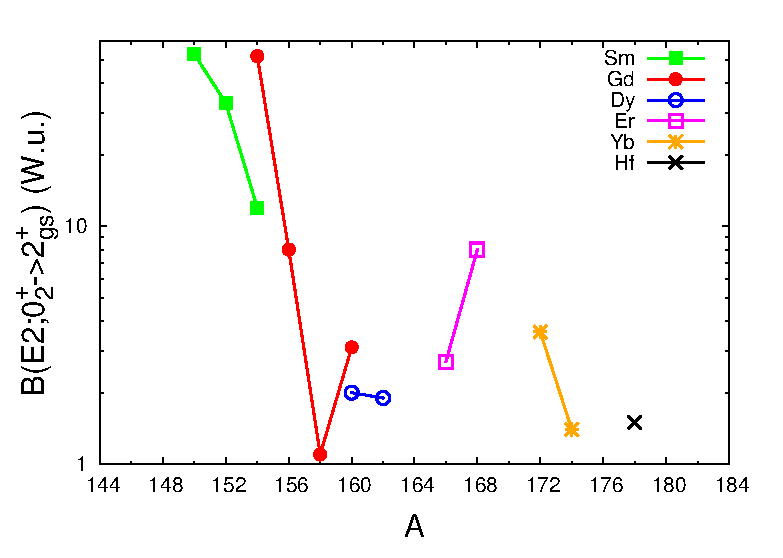
\includegraphics[width=0.88\textwidth]{figures/Rare_Earth_02_BE2.eps}\\
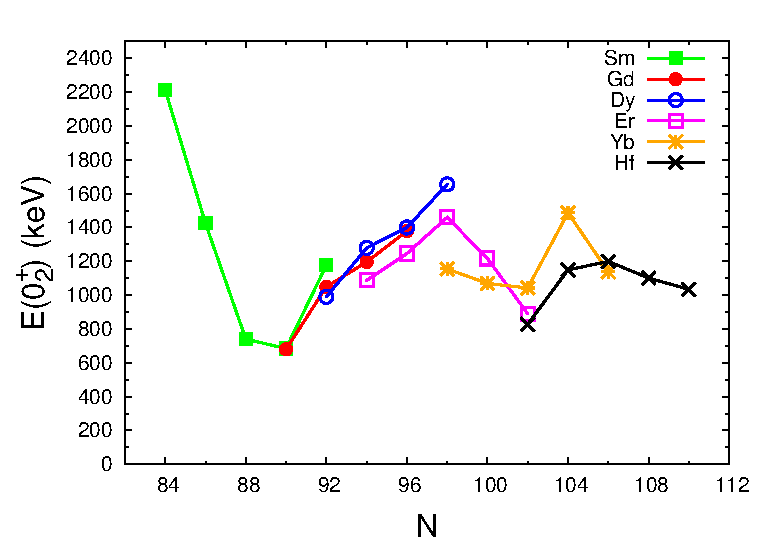
\includegraphics[width=0.88\textwidth]{figures/Rare_Earth_0s_N.eps}\\
\end{center}
\caption{Absolute B(E2;0$^+_2\rightarrow$2$^+_{gs}$) (in Weisskopf units) measurements for rare-earth nuclei, showing the scattered experimental data that spans an order of magnitude variance. The bottom plot shows the energy of the 0$^+_2$ bandheads as a function of N, which shows a slightly more variant energy systematic than the 2$^+$ bandheads. \label{fig:Rare_Earth_02_BE2}}
\end{figure}

The emergence of the nuclear data that gives this unclear picture (particularly of the scattered B(E2) strengths) has garnered significant skepticism of \textit{any} vibrational degrees of freedom in the nucleus \cite{Garrett_betavib2001}. The story is \textit{still} unclear on the nature of any vibrational states in deformed nuclei due to the incomplete data surrounding it; if any clarification is to be made, we need lifetime information to say one way or the other.


By a similar merit for the octupole vibration, in Figure \ref{fig:phonon_def} we see the split quartet of low-lying negative parity states, as expected, yet these $\lambda$=3 excitations are not as well studied as their quadrupole counterparts \cite{Casten_text}. Several different phenomena occur in the low-lying negative parity states of deformed nuclei, including an inversion in the energy ordering of states as N increases, irregularities among the transition probabilities (as a function of $\Delta$K) throughout the rare-earth region of nuclei, among others \cite{Borner_collective1999,Casten_text}. Continue the multipole expansion to higher-order terms, and the hexadecapole ($\lambda$=4) vibrations appear. Again, we state here that these negative parity states and higher-order vibrational phonons have not seen the same order of experimental rigor and study as their $\lambda$=2 counterparts have; this work hopes to aid in the lack of vital lifetime information on low-lying negative parity states in the deformed region of nuclei. Systematic behavior of negative parity states (as well as the strength of quadrupole vibrations) varies wildly across the entire rare-earth region of nuclei and have been caught in the epicenter of experimental focus in nuclear structure in the past several decades. 

Much like the quadrupole counterparts, we can also picture a structure of coupled quadrupole-octupole-type phonons to either octupole or quadrupole phonons, further increasing the possible K-projections available to study \cite{Pascu_octupole_2015}. For example, a 2$^+\otimes$3$^-$ coupling can produce projections of 1$^-$, 2$^-$, 3$^-$, 4$^-$ \& 5$^-$, if we follow the same parity and algebraic combination rules inherent to deformed quantum systems. 

% In terms of the IBA, particular energetics and selection rules emerge from each dynamical symmetry that govern the overall behavior of the nuclear structure. For example, a pure SU(3) deformed rotator has specific ratios of reduced transition probabilities expected, as well as an expected grouping of K=0,2 excited bands inside of the same irreduceable representation \cite{Casten_text}. For example (and in stark contrast to the geometric model where they are discrete types of vibration), the K=0 band is interpreted as an excitation built on top of the K=2 $\gamma$-vibrational band, where we would expect to observe strong transitions between the bands, with weak transitions to the ground state band.
%outline some IBA symmetries and expected B(E2)'s or whatever
%The Pauli principle has a profound effect on the evolution of nuclear structure; energies of excited states and branching ratios are affected by the pairing of nucleons




